\documentclass[letterpaper]{article} \usepackage[submission]{aaai2027} \usepackage[hyphens]{url} \usepackage{graphicx} \usepackage{subcaption} \urlstyle{rm} \def\UrlFont{\rm} \usepackage{natbib} \usepackage{amsmath} \usepackage{amssymb} \usepackage{booktabs} \usepackage{multirow} \usepackage{algorithm} \usepackage{algorithmic}

\newcommand{\cmark}{$\checkmark$}
\newcommand{\xmark}{$\times$}

\frenchspacing \setlength{\pdfpagewidth}{8.5in} \setlength{\pdfpageheight}{11in} \setcounter{secnumdepth}{0}

\pdfinfo{/TemplateVersion (2027.1)}

\title{ShapeShift: Active-Shape Scheduling for Long-Context Diffusion Language Model Serving}
\author{Anonymous Authors}
\affiliations{}

\begin{document}
\maketitle

\begin{abstract}
Diffusion language models (dLLMs) generate by repeatedly updating a prompt-response canvas rather than extending a cached prefix one token at a time. This execution model creates a serving bottleneck that is easy to miss in single-request inference: when short and long requests share a denoising step, the transformer body runs at the longest sequence shape, so shorter requests repeatedly pay padding work created by their batch companions. We identify this effect as \emph{long-context shape waste} and show that it is an online scheduling problem. We present \emph{ShapeShift}, an active-shape continuous batching runtime that treats sequence length as a step-level scheduling resource. ShapeShift chooses an anchor request, fills the step batch with nearest-length companions, filters additions that would create excessive rectangular work, and uses service-gap aging to keep old or shape-outlier requests in service. Integrated into dlmserve, ShapeShift improves online throughput by 1.19--1.49$\times$ over FCFS on mixed-length serving traces, while reducing mean and p95 request latency. Longer-horizon validation across five workloads shows 1.14--1.88$\times$ throughput gains. The gains concentrate in the predicted regime: backlogged, shape-heterogeneous ready pools where active step-batch selection can prevent repeated long-shape co-residence.
\end{abstract}

\section{Introduction}

Autoregressive (AR) LLMs have become the default engine behind interactive assistants and production text services, but their left-to-right decoding keeps generation fundamentally sequential at the token level. Diffusion language models (dLLMs) offer a different contract: they allocate a response canvas, initialize unknown positions with mask tokens, and repeatedly denoise the prompt-response canvas with a bidirectional transformer. Recent models and systems, including LLaDA, Dream, LLaDA2.0, Fast-dLLM, dInfer, and dLLM-Serve~\cite{nie2025llada,dream2025,llada20_2025,zhao2025fastdllm,dInfer2025,dllmserve2025}, show growing interest in this model family. Moving dLLMs from single-request inference to shared serving, however, exposes a batching problem specific to repeated full-canvas updates: each denoising step revisits the full canvas, so a short request batched with a long request can repeatedly inherit the long request's sequence shape.

Existing serving optimizations attack adjacent bottlenecks. AR long-context systems optimize prefill/decode separation, KV-cache placement, sequence parallelism, and length-aware prefill or decode scheduling~\cite{loongserve2024,alignedserve2026,laps2026}. Their scheduling objective follows AR execution: pay the prompt once, then advance cached requests incrementally. Recent dLLM inference and serving systems reduce the cost of executing a denoising step through cache reuse, parallel decoding, sparse attention, or phase scheduling~\cite{zhao2025fastdllm,dInfer2025,dllmserve2025}. These techniques make a chosen update cheaper, while the serving loop still determines which active requests create the update shape. Thus an online dLLM server can waste transformer-body work by repeatedly co-scheduling long and short canvases in the same denoising batch.

Our key observation is that this waste is a scheduling effect. In GPU probes across three dLLM checkpoints, mixed short/long batches take essentially the same time as all-long batches over the same denoising steps. Once a long request enters a step batch, every shorter companion is charged for the long rectangular shape at each co-scheduled step. We call this effect \emph{long-context shape waste}. It changes the runtime interpretation of sequence length: length is not only an admission-time property, but a repeated-step resource that should be controlled whenever the active set is rebatched.

This view shifts the serving question from ``how fast can the next update run?'' to ``which active sequence shapes should run together?'' The distinction matters because an update can be locally optimized by kernels or caches while still being globally inefficient for the ready pool if its batch shape is dominated by a long outlier. ShapeShift targets this missing active-set decision.

We design \emph{ShapeShift}, an active-shape scheduler for dLLM continuous batching. ShapeShift makes one local decision at each scheduler tick: which ready requests should share the next denoising step. It chooses an anchor request to define the length region of the step, fills with nearest-length companions to reduce rectangular padding, filters candidates that would create excessive padded work, and promotes overdue requests through service-gap aging. These rules are deliberately step-level rather than admission-level: a request may need different companions as other requests arrive, finish, or become overdue.

We integrate ShapeShift into dlmserve and evaluate it with direct online arrivals from serving-oriented workloads, including ShareGPT long-context chat, Wikipedia-style multi-hop QA, instruction mixes, and heterogeneous multi-task queues. The evaluation follows the mechanism: cross-model runs measure end-to-end serving gains, ablations separate active-shape batching from compactness and aging controls, and boundary sweeps identify when the ready pool contains enough backlog and length diversity for shape-compatible batching.

This paper makes the following contributions.

\begin{enumerate}
  \item We identify \emph{long-context shape waste}: in dLLM serving, short requests can repeatedly pay the transformer-body cost of the longest request in their denoising step batch.
  \item We design and implement \emph{ShapeShift}, a step-level scheduler that combines anchor-based nearest-length batching, compactness filtering, and service-gap aging to control padding while preserving regular service for unusual-length requests.
  \item We evaluate ShapeShift on online dLLM serving workloads across four open checkpoints, showing up to 2.15$\times$ throughput improvement over FCFS with lower mean and p95 latency, and characterize the backlog and heterogeneity regimes where active-shape scheduling is most effective.
\end{enumerate}

\section{Background and Motivation}

\subsection{Step Batches and Rectangular Shape}

Let a request have prompt length $P$, generation canvas length $G$, and total sequence length $L=P+G$. A dLLM denoising step runs the transformer over the current prompt-response canvas, whose unknown output positions are represented by mask tokens. For serving, the important property is that each step processes the whole canvas rather than appending one token to a cached prefix.

When a server batches multiple active requests at a denoising step, the requests must share a common sequence dimension. A step batch $\mathcal{B}$ is therefore padded to its longest member and executes as a rectangle with token-row size
\[
  |\mathcal{B}|\cdot L_{\max}(\mathcal{B}), \quad
  L_{\max}(\mathcal{B})=\max_{r\in\mathcal{B}} L_r .
\]
Only $\sum_{r\in\mathcal{B}} L_r$ token rows correspond to actual request content. We use the shape-padding ratio
\[
  \rho(\mathcal{B}) =
  \frac{|\mathcal{B}|\cdot L_{\max}(\mathcal{B})}
       {\sum_{r\in\mathcal{B}} L_r}
\]
as a scheduler-facing proxy for avoidable rectangular work. The metric captures the part of step cost that changes when the scheduler changes which canvases co-reside; the same-protocol experiments keep model kernels and generation settings fixed.

\subsection{Why Shape Matters Repeatedly}

Length-aware scheduling already appears in AR serving, but dLLMs amplify the consequence of poor length pairing. In AR serving, a long prompt mainly increases prefill cost; later decode iterations reuse a KV cache and add one token per request. In a dLLM, the same prompt-response canvas is revisited over many denoising steps. If a 2K-token request is repeatedly batched with much shorter requests, those shorter requests repeatedly execute under the 2K-token rectangular shape.

This repeated shape effect separates model-side dLLM acceleration from serving-side scheduling. Cache reuse, sparse attention, and parallel decoding reduce the cost of a chosen step, while active-shape scheduling decides which ready requests create that step shape. FCFS is a natural online baseline because it preserves arrival order, but its ordering rule is unrelated to shape compatibility. The scheduler therefore needs a second notion of locality beyond arrival time: which active canvases should co-reside in the next rectangular step.

\begin{figure*}[t]
  \centering
  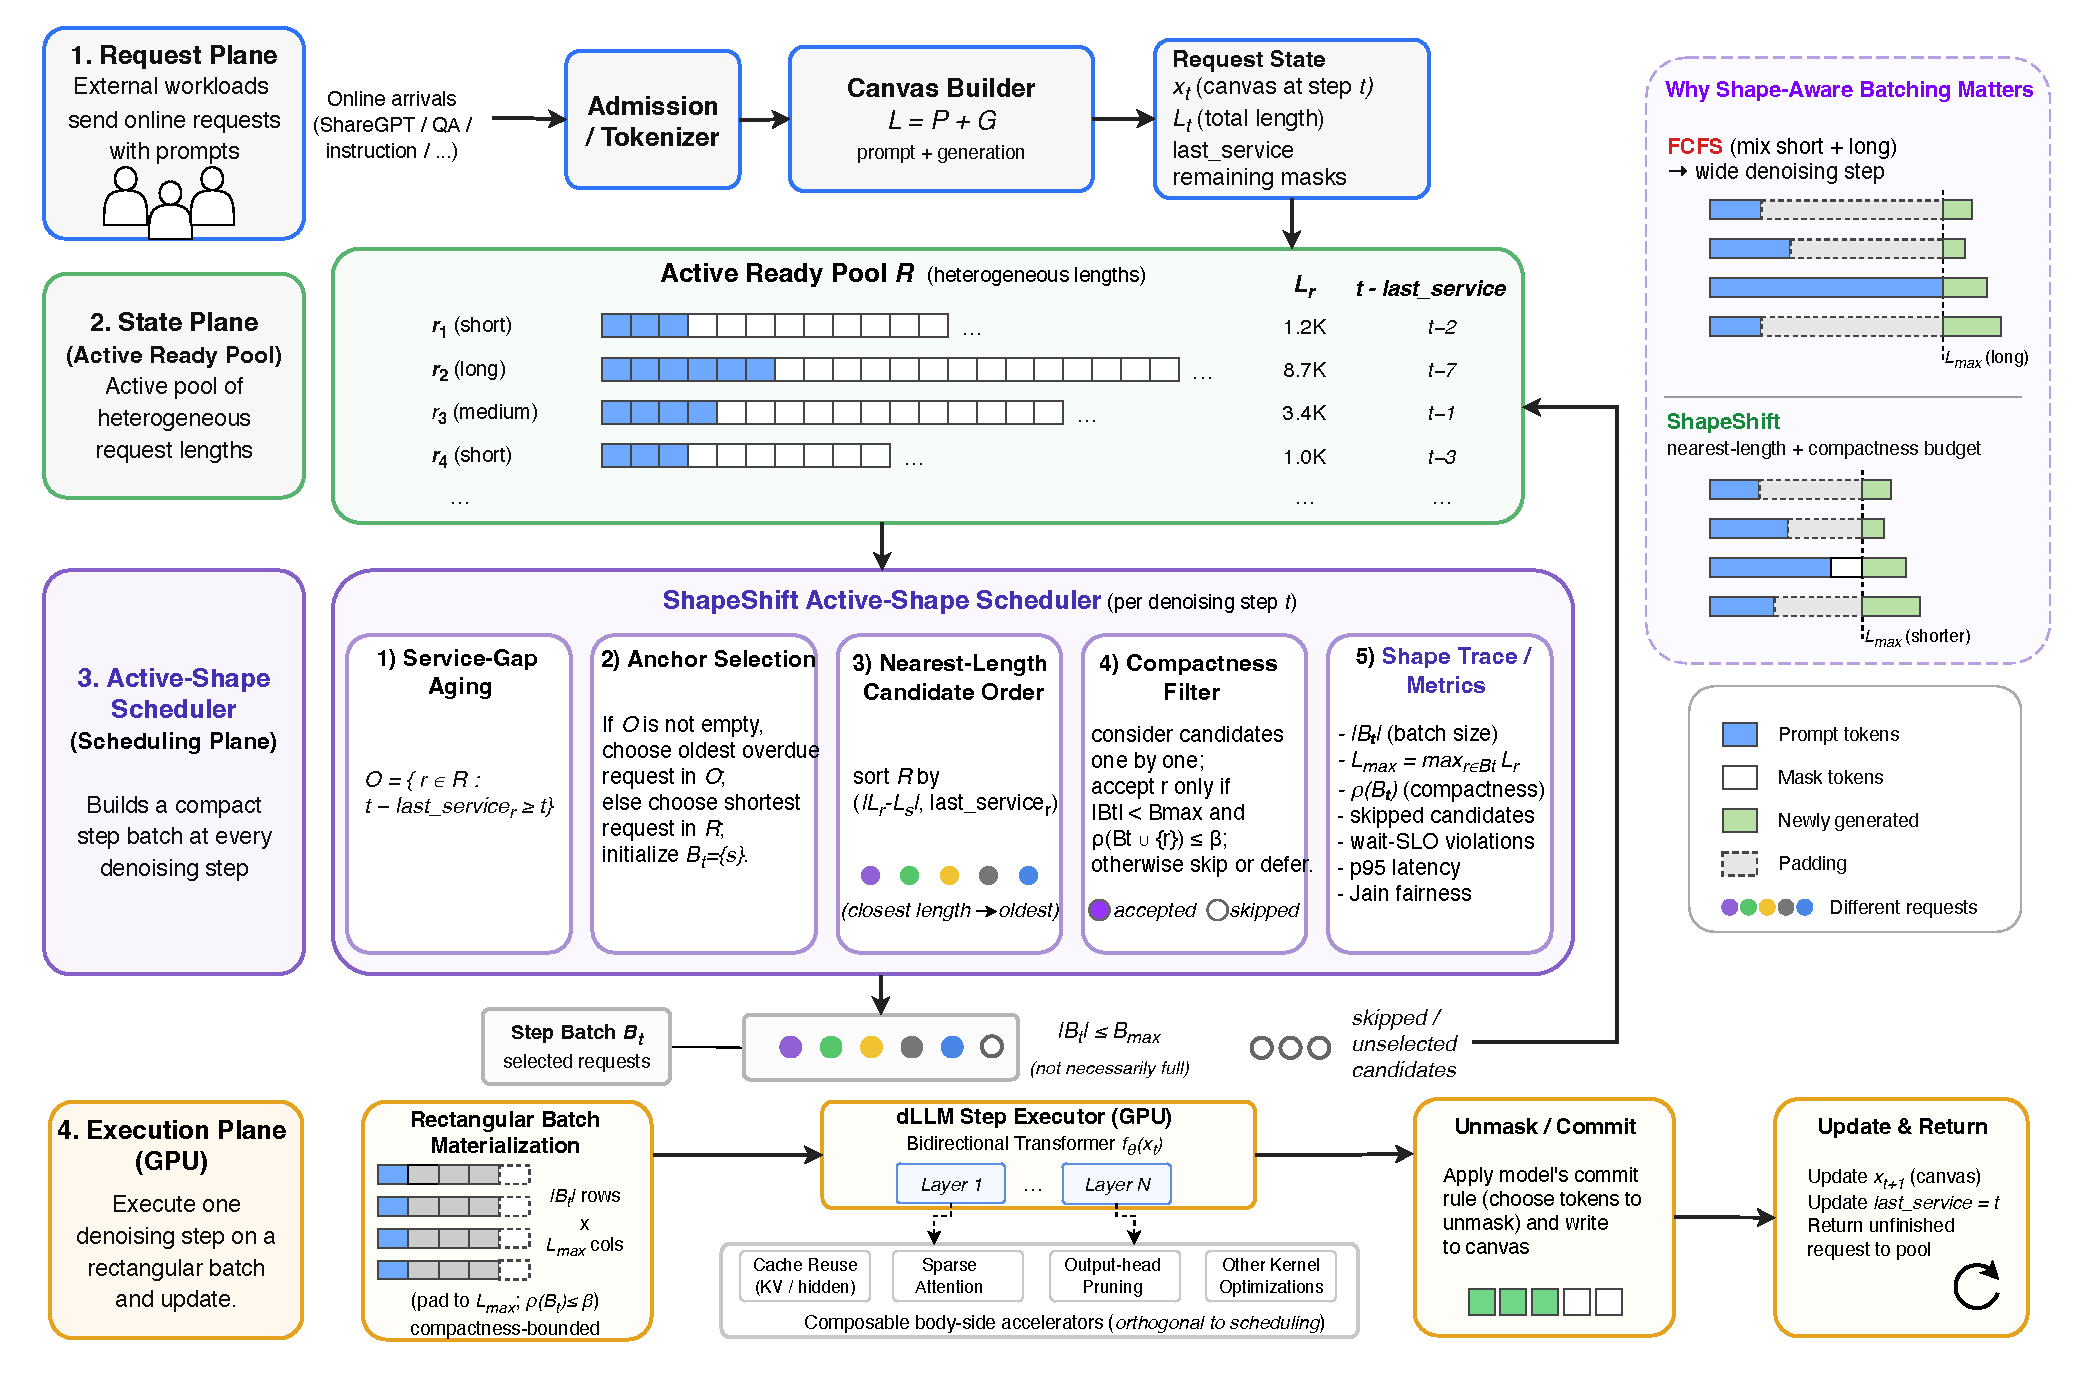
\includegraphics[width=0.9\linewidth]{figures/ShapeShift-Arch.pdf}
  \caption{ShapeShift serving loop and active-shape scheduler for step-level dLLM batching.}
  \label{fig:design-overview}
  \vspace{-0.5em}
\end{figure*}

\subsection{Motivating Observations}

\textbf{Observation 1: online dLLM traces are shape-heterogeneous.} We build length traces from ShareGPT using the LLaDA tokenizer. Single-turn requests are mostly short but have a long tail, while multiturn accumulated requests often approach the serving-window limit. This spread creates a scheduling opportunity: FCFS can repeatedly pull short requests up to tail shapes, while shape-aware scheduling can group compatible canvases.

\textbf{Observation 2: mixed-length batches behave like long batches.} We probe three dLLM checkpoints with real model execution and a fixed output canvas. Table~\ref{tab:motivation-probe} reports latency for this controlled probe. Across checkpoints, the mixed short/long batch is nearly as expensive as the all-long batch. Once short requests are paired with long contexts, their short sequence length largely disappears from transformer-body cost.

\begin{table}[t]
\centering
\scriptsize
\setlength{\tabcolsep}{2.8pt}
\begin{tabular}{lcccc}
\toprule
Model & All short & All long & Mixed & Mix/long \\
\midrule
LLaDA-8B~\cite{nie2025llada} & 1.604s & 11.680s & 11.671s & 1.00$\times$ \\
Dream-7B~\cite{dream2025} & 1.387s & 10.179s & 10.174s & 1.00$\times$ \\
CoDA-1.7B~\cite{coda2025} & 0.474s & 3.491s & 3.511s & 1.01$\times$ \\
\bottomrule
\end{tabular}
\caption{GPU probe latency for short, long, and mixed-length dLLM batches.}
\label{tab:motivation-probe}
\end{table}

Together, these observations turn length heterogeneity into a serving decision. A scheduler should choose companions at step granularity because the active set changes as requests arrive, finish, and advance through denoising. It should prefer shape-compatible companions because rectangular padding is paid by every request in the step. It should also keep long or unusual-length requests in service, since a purely compact policy can defer requests that lack nearby companions. ShapeShift is organized around these requirements.

\section{Design}

\subsection{Overview and Abstraction}

ShapeShift is a runtime scheduling layer for active dLLM requests. It leaves the denoising rule and model kernels unchanged, and instead decides which unfinished requests share each denoising step. Figure~\ref{fig:design-overview} summarizes the serving loop. Requests arrive online, are tokenized, and receive a prompt-response canvas of length $L=P+G$. The runtime stores each unfinished request in an active ready pool $R$ together with its current canvas state $x_t$, total length $L_r$, last service time, and remaining masks. At scheduler tick $t$, ShapeShift selects a step batch $\mathcal{B}_t\subseteq R$; the engine materializes a rectangular batch, runs one dLLM step on the GPU, commits newly unmasked tokens, and returns unfinished requests to the ready pool.

The scheduler controls the rectangular execution shape $(|\mathcal{B}_t|,L_t^{\max})$, where $L_t^{\max}=\max_{r\in\mathcal{B}_t}L_r$. The right side of Figure~\ref{fig:design-overview} illustrates why this matters: FCFS can mix short and long canvases, forcing every row to pad to the long request, whereas ShapeShift builds a compact step batch whose $L_t^{\max}$ is closer to the selected requests' useful lengths. ShapeShift implements this choice with five local blocks shown in the scheduler plane of the figure: service-gap aging, anchor selection, nearest-length candidate ordering, compactness filtering, and shape tracing.

This objective differs from ordinary admission bucketing. A request remains active for many denoising steps, and its best companions can change as other requests arrive, complete, or become overdue. ShapeShift therefore rebatches at step granularity rather than binding a request to a fixed admission bucket. The policy makes the next step compact enough to execute efficiently while keeping a path for old or unusual-length requests to be selected.

ShapeShift maintains three scheduler invariants. First, the selected batch should be locally shape-compact, so the longest row in the rectangle is close to the useful work in the batch. Second, the active set should be reconsidered at every step, because arrivals and completions continuously change which companions are available. Third, shape compactness should be bounded by service regularity: a request that lacks nearby companions must still re-enter service. The anchor, fill, compactness, and aging rules below implement these invariants with local queue state.

\subsection{Service-Gap Anchoring}

ShapeShift first chooses an anchor request $s$. The anchor is the scheduler's local commitment to a length region: once $s$ is chosen, the rest of the batch is built around requests close to $L_s$. A shortest-first anchor usually produces compact batches under backlog, but it can delay long or unusual lengths. An oldest-first anchor improves service regularity, but it can repeatedly pull short requests into long rectangular shapes. ShapeShift uses a service-gap budget $\tau$ to switch between these behaviors.

Let $r.\mathrm{last\_service}$ be the last scheduler time at which request $r$ received a denoising step. ShapeShift forms the overdue set
\[
  O=\{r\in R: t-r.\mathrm{last\_service}\ge \tau\}.
\]
If $O$ is non-empty, the oldest overdue request becomes the anchor; otherwise, the shortest ready request becomes the anchor. This rule corresponds to the service-gap aging and anchor-selection blocks in Figure~\ref{fig:design-overview}. The budget acts as a runtime service-regularity knob: compact batches remain the default, while overdue requests regain anchor priority before compactness turns into indefinite deferral.

\subsection{Nearest-Length Fill with Compactness Filtering}

After choosing anchor $s$, ShapeShift ranks candidates by $|L_r-L_s|$ and considers them in that order, using last-service time as a stable tie-breaker. This nearest-length order targets the mechanism directly: if companions have lengths close to $L_s$, then $L_t^{\max}$ stays close to the useful token rows in the batch.

Nearest-length fill alone is not enough. Under a thin or skewed ready pool, the next nearest request may still be much longer than the current candidates; adding it can increase padded work more than it increases useful work. ShapeShift therefore admits a companion only if the resulting batch satisfies a compactness budget. We write the budget as a padding-ratio constraint,
\[
  \rho(\mathcal{B}\cup\{r\}) \le \beta,
\]
although an implementation can enforce the same idea through a rectangular token-row limit,
\[
  |\mathcal{B}\cup\{r\}|\cdot \max_{u\in\mathcal{B}\cup\{r\}} L_u \le C.
\]
Requests that fail the compactness test remain in the ready pool, where they may become good companions for a later anchor or become overdue and receive service through aging. Compactness filtering is therefore a step-batch decision rather than an admission decision. The runtime records $(|\mathcal{B}|,L_t^{\max},\rho)$ for each step so the evaluation can connect end-to-end throughput changes to concrete shape decisions.

\subsection{Execution and Rebatching Loop}

The selected batch $\mathcal{B}_t$ is not necessarily full. If adding another candidate would violate the compactness budget, ShapeShift prefers an underfilled but compact rectangular step over a full but highly padded one. The execution plane in Figure~\ref{fig:design-overview} shows the resulting flow: materialize rows for $\mathcal{B}_t$, pad to $L_t^{\max}$, run one bidirectional transformer step, apply the model's commit rule, update $x_{t+1}$ and last-service time, and return unfinished requests to $R$.

This step-level loop is what makes ShapeShift different from static length bucketing. A short request may share a long shape in one step, then recover a compact shape after the long request completes or after new short companions arrive. A deferred long request remains visible in the ready pool and eventually becomes an aging anchor. Active-shape scheduling therefore adapts to the changing request set rather than making a one-time admission decision.

Algorithm~\ref{alg:shapeshift} instantiates the policy. The tie-breaker by last-service time keeps the fill rule stable when several requests have the same length distance to the anchor. The evaluation measures the service-gap budget through request latency and inter-service gaps.

\begin{algorithm}[t]
\caption{ShapeShift Active-Shape Step Scheduler}
\label{alg:shapeshift}
\begin{algorithmic}[1]
\STATE \textbf{Input:} ready set $R$, batch size $B$, time $t$, service-gap budget $\tau$, compactness budget $\beta$
\STATE $O \leftarrow \{r\in R: t-r.\mathrm{last\_service}\ge \tau\}$
\IF{$O$ is not empty}
  \STATE $s \leftarrow$ oldest request in $O$
\ELSE
  \STATE $s \leftarrow$ shortest request in $R$
\ENDIF
\STATE $\mathcal{B}\leftarrow \{s\}$
\STATE Sort $R\setminus\{s\}$ by $(|L_r-L_s|, \mathrm{last\_service}_r)$
\FOR{each $r$ in sorted order}
  \IF{$|\mathcal{B}|<B$ and $\rho(\mathcal{B}\cup\{r\})\le\beta$}
    \STATE $\mathcal{B}\leftarrow\mathcal{B}\cup\{r\}$
  \ENDIF
\ENDFOR
\STATE Record $(|\mathcal{B}|,\max_{r\in\mathcal{B}}L_r,\rho(\mathcal{B}))$
\STATE Set $r.\mathrm{last\_service}\leftarrow t$ for $r\in\mathcal{B}$
\STATE Return $\mathcal{B}$
\end{algorithmic}
\end{algorithm}

This policy organizes the ablations used in the evaluation. FCFS uses the oldest request and fills by arrival order, preserving implicit fairness but ignoring shape. ShapeShift-Shape uses shortest-by-length anchoring and nearest-length fill without compactness or service-gap controls; it isolates the utilization effect of active-shape batching. ShapeShift-Aging adds the service-gap anchor rule but omits the compactness budget; it isolates the service-regularity control. Full ShapeShift combines active-shape batching, compactness filtering, and service-gap aging.

\subsection{Runtime Scope and Composition}

ShapeShift runs after admission, so its control surface is the active ready pool. This makes the operating regime precise: the scheduler is strongest when the ready pool is both backlogged and length-heterogeneous, while thin queues provide fewer shape-compatible companions.

ShapeShift composes with model-side and output-side acceleration. Cache reuse, sparse attention, and output-head pruning reduce the cost of executing a chosen step batch; ShapeShift decides which requests share that batch. This separation is why the same scheduler can wrap dlmserve directly and can also be tested around an adjacent dInfer-backed execution path.

\begin{figure*}[t]
  \centering
  \begin{subfigure}[t]{0.24\textwidth}
    \centering
    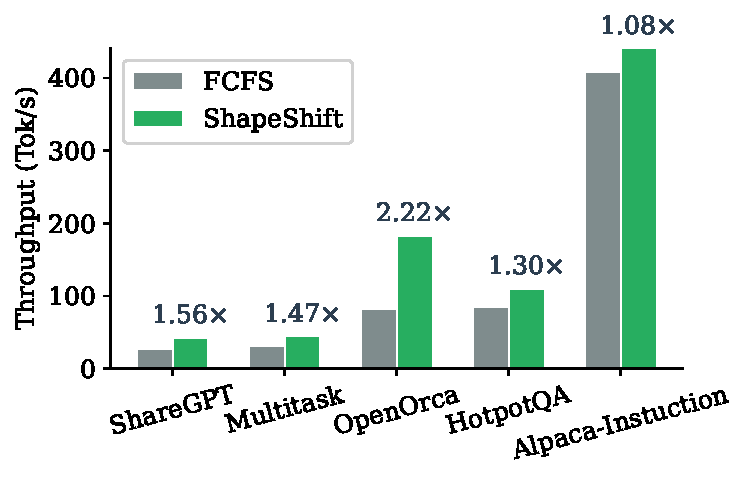
\includegraphics[width=\linewidth]{figures/bar_llada8b_throughput.pdf}
    \caption{LLaDA-8B}
    \label{fig:main-throughput-llada8b}
  \end{subfigure}\hfill
  \begin{subfigure}[t]{0.24\textwidth}
    \centering
    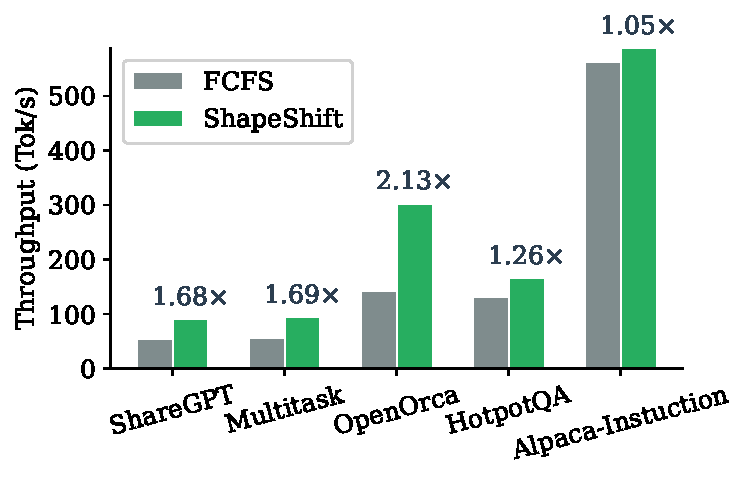
\includegraphics[width=\linewidth]{figures/bar_dream7b_throughput.pdf}
    \caption{Dream-7B}
    \label{fig:main-throughput-dream7b}
  \end{subfigure}
  \vspace{0.6em}
  \begin{subfigure}[t]{0.24\textwidth}
    \centering
    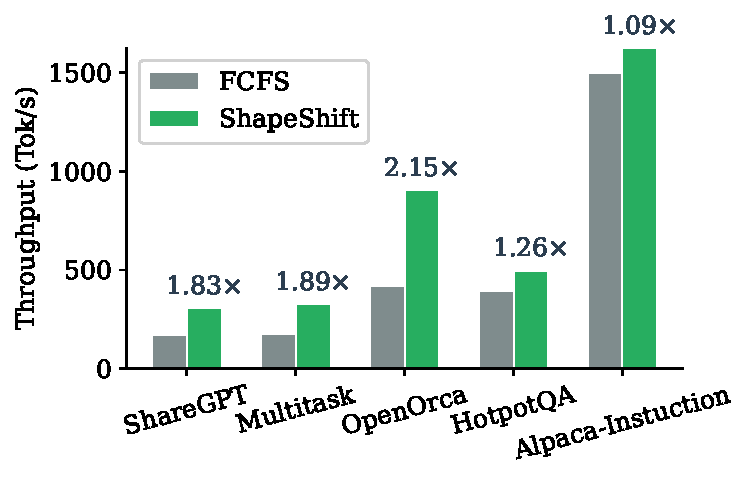
\includegraphics[width=\linewidth]{figures/bar_coda17b_throughput.pdf}
    \caption{CoDA-1.7B}
    \label{fig:main-throughput-coda17b}
  \end{subfigure}\hfill
  \begin{subfigure}[t]{0.24\textwidth}
    \centering
    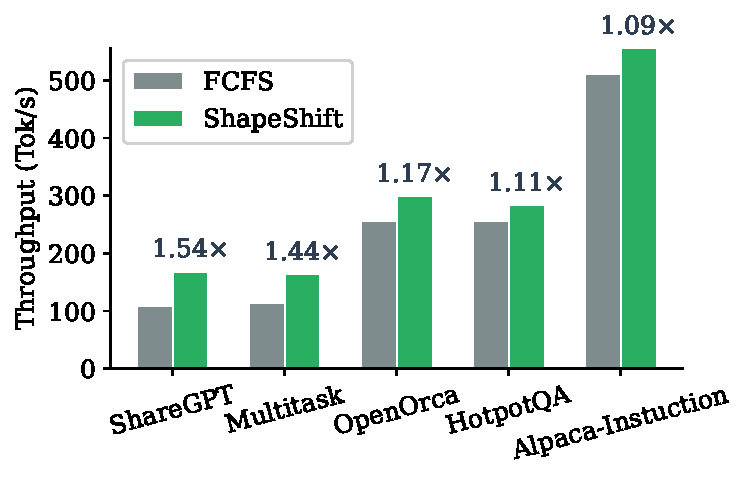
\includegraphics[width=\linewidth]{figures/bar_llada2mini_throughput.pdf}
    \caption{LLaDA2.0-mini}
    \label{fig:main-throughput-llada2mini}
  \end{subfigure}
  \caption{Online serving throughput on mixed-length workloads across four dLLM checkpoints.}
  \label{fig:main-throughput}
  \vspace{-0.5em}
  \end{figure*}
  
  \begin{figure*}[t]
  \centering
  \begin{subfigure}[t]{0.24\textwidth}
    \centering
    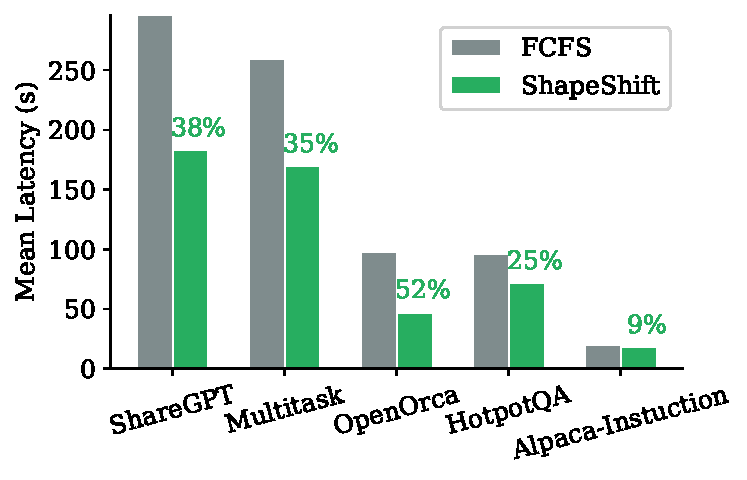
\includegraphics[width=\linewidth]{figures/bar_llada8b_mean.pdf}
    \caption{LLaDA-8B}
    \label{fig:main-mean-llada8b}
  \end{subfigure}\hfill
  \begin{subfigure}[t]{0.24\textwidth}
    \centering
    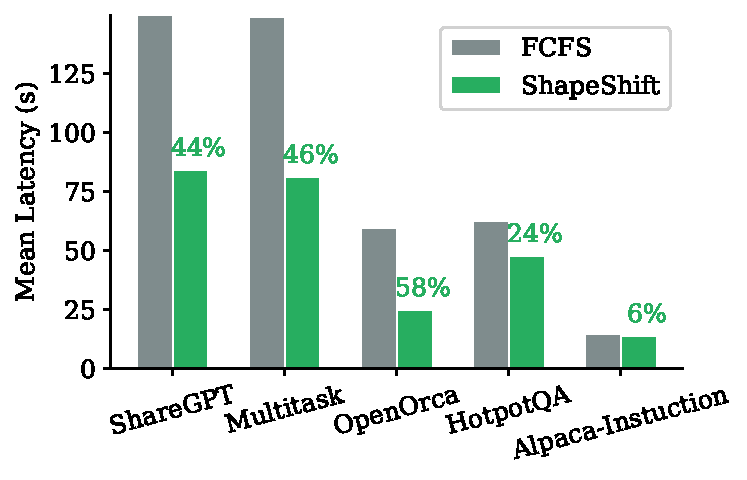
\includegraphics[width=\linewidth]{figures/bar_dream7b_mean.pdf}
    \caption{Dream-7B}
    \label{fig:main-mean-dream7b}
  \end{subfigure}
  \vspace{0.6em}
  \begin{subfigure}[t]{0.24\textwidth}
    \centering
    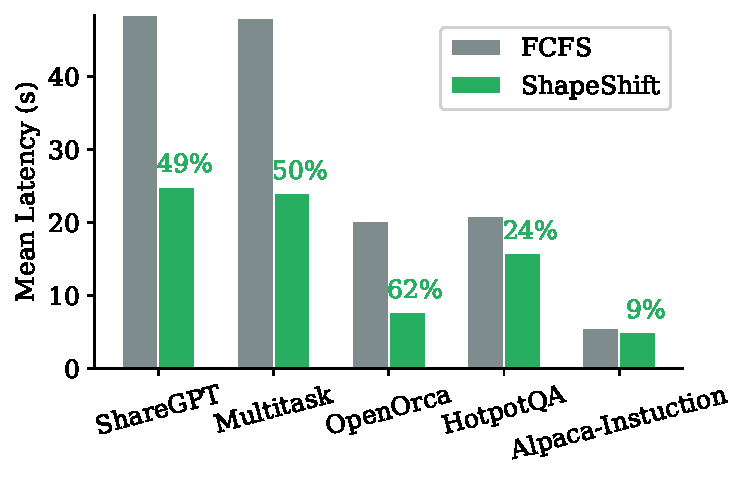
\includegraphics[width=\linewidth]{figures/bar_coda17b_mean.pdf}
    \caption{CoDA-1.7B}
    \label{fig:main-mean-coda17b}
  \end{subfigure}\hfill
  \begin{subfigure}[t]{0.24\textwidth}
    \centering
    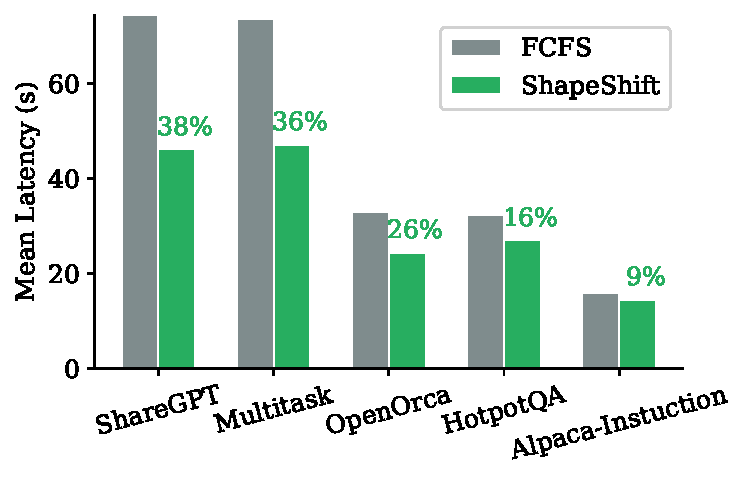
\includegraphics[width=\linewidth]{figures/bar_llada2mini_mean.pdf}
    \caption{LLaDA2.0-mini}
    \label{fig:main-mean-llada2mini}
  \end{subfigure}
  \caption{Mean request latency on mixed-length online serving workloads across four dLLM checkpoints.}
  \label{fig:main-mean}
  \vspace{-0.5em}
  \end{figure*}
  
  \begin{figure*}[t]
  \centering
  \begin{subfigure}[t]{0.24\textwidth}
    \centering
    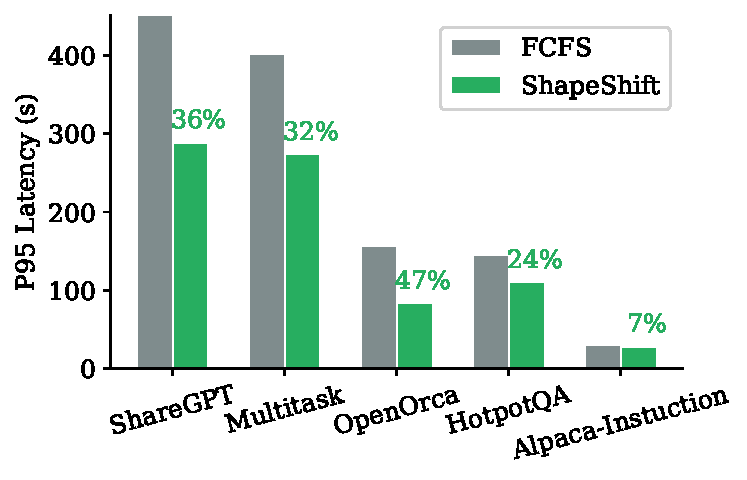
\includegraphics[width=\linewidth]{figures/bar_llada8b_p95.pdf}
    \caption{LLaDA-8B}
    \label{fig:main-p95-llada8b}
  \end{subfigure}\hfill
  \begin{subfigure}[t]{0.24\textwidth}
    \centering
    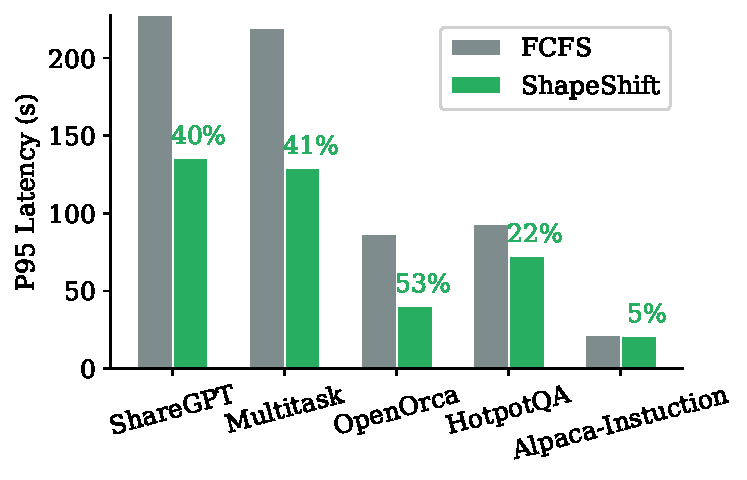
\includegraphics[width=\linewidth]{figures/bar_dream7b_p95.pdf}
    \caption{Dream-7B}
    \label{fig:main-p95-dream7b}
  \end{subfigure}
  \vspace{0.6em}
  \begin{subfigure}[t]{0.24\textwidth}
    \centering
    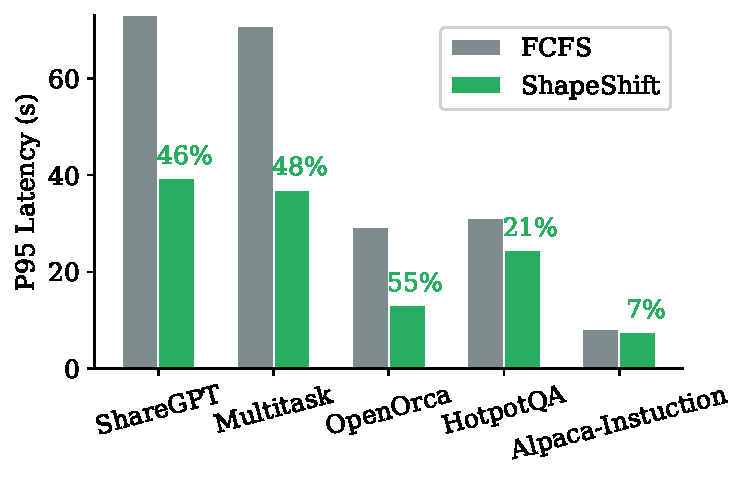
\includegraphics[width=\linewidth]{figures/bar_coda17b_p95.pdf}
    \caption{CoDA-1.7B}
    \label{fig:main-p95-coda17b}
  \end{subfigure}\hfill
  \begin{subfigure}[t]{0.24\textwidth}
    \centering
    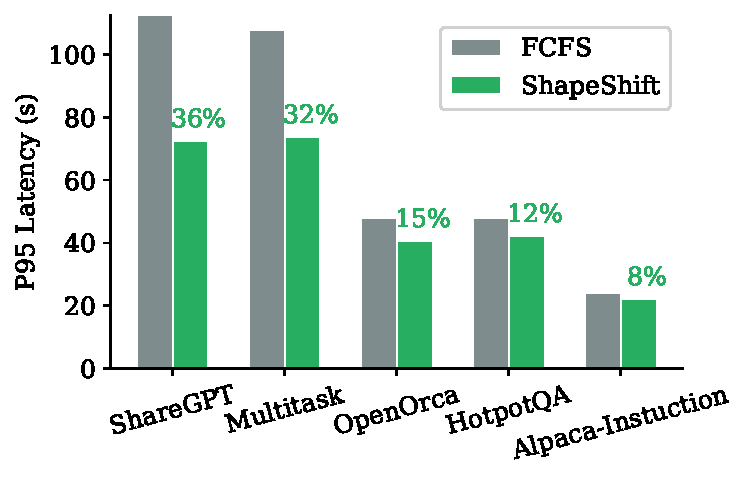
\includegraphics[width=\linewidth]{figures/bar_llada2mini_p95.pdf}
    \caption{LLaDA2.0-mini}
    \label{fig:main-p95-llada2mini}
  \end{subfigure}
  \caption{P95 request latency on mixed-length online serving workloads across four dLLM checkpoints.}
  \label{fig:main-p95}
  \vspace{-0.5em}
  \end{figure*}
  

\section{Evaluation}

We evaluate ShapeShift by following the paper's central claim: repeated sequence-shape waste is a scheduling bottleneck in online dLLM serving, and active-shape step batching reduces that waste. The experiments first compare ShapeShift against the unmodified FCFS scheduler in the same dlmserve execution path, then test whether the scheduler composes with a dInfer-backed generation path, and finally connect the gains to padding ratios, ablations, backlog, and length heterogeneity.

\subsection{Experimental Setup}

Main results use dlmserve~\cite{dlmserve2026}, a recent open-source text dLLM serving engine with step-level continuous batching. We compare against its default FCFS step scheduler while keeping the model, kernels, output setting, and maximum batch capacity fixed. Experiments run on a single NVIDIA RTX A6000 GPU with 48GB memory.

The main workloads are length traces tokenized with the LLaDA tokenizer: ShareGPT multiturn chat, HotpotQA/Wikipedia-style multi-hop QA, a multi-task mix containing short chat, long chat, and Wikipedia QA requests, and a ShareGPT short/long mixture. FCFS on LLaDA-8B is the same-model online scheduler baseline; Dream, CoDA, and LLaDA2.0-mini repeat that comparison for cross-model robustness. The dInfer wrapper appears as an adjacent composition check, while the main latency figures remain within the same dlmserve online protocol.

We use consistent policy names across all tables. ShapeShift-Shape isolates nearest-length active-shape batching; ShapeShift-Aging adds service-gap anchoring; full ShapeShift combines active-shape batching, compactness filtering, and service-gap aging. We report completed-token throughput, mean request latency, and p95 request latency under online arrivals.

\subsection{Main Online Serving Results}

Figures~\ref{fig:main-throughput},~\ref{fig:main-mean}, and~\ref{fig:main-p95} summarize the primary online serving evidence. Across four mixed-length workloads and four open dLLM checkpoints, ShapeShift improves throughput while also reducing mean and p95 request latency relative to FCFS. The throughput gains are consistent across model sizes, indicating that the scheduler is exploiting a serving-level shape effect rather than a checkpoint-specific artifact. Mean latency improves because compact step batches reduce repeated padded transformer work, and p95 latency also drops because service-gap aging keeps shape clustering from turning into long-tail deferral. The improvement is strongest on workloads with long-context spread, where FCFS repeatedly forms rectangular batches around tail-length requests.

The latency trends are important for interpreting the throughput gains. ShapeShift is not simply filling the GPU with more work while shifting delay to unlucky requests; throughput improves while both mean and tail latency decrease. This indicates that active-shape batching reduces the amount of work each request repeatedly shares with incompatible companions. The cross-checkpoint pattern also suggests that the opportunity comes from the rectangular serving geometry of dLLM steps, not from a special property of one model implementation.

\subsection{Composition with dInfer}

dInfer~\cite{dInfer2025} and Fast-dLLM~\cite{zhao2025fastdllm} target the dLLM generation body, while ShapeShift schedules which requests share repeated denoising batches. Figure~\ref{fig:dinfer-wrapper} tests this separation by placing ShapeShift around a dInfer-backed online wrapper. The wrapper is synchronous and executes one selected batch to completion before selecting the next batch, so the absolute latencies are not directly comparable to dlmserve. The comparison within the wrapper is still meaningful: FCFS and ShapeShift use the same dInfer generation path and differ only in request grouping.

\begin{figure*}[t]
\centering
\begin{subfigure}[t]{0.3\textwidth}
  \centering
  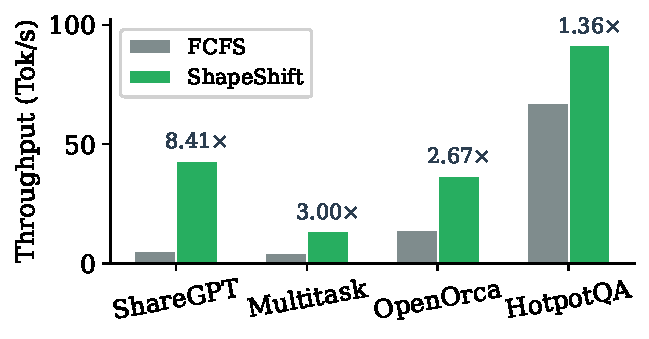
\includegraphics[width=\linewidth]{figures/bar_dinfer_wrapper_throughput.pdf}
  \caption{Throughput}
  \label{fig:dinfer-wrapper-throughput}
\end{subfigure}\hfill
\begin{subfigure}[t]{0.3\textwidth}
  \centering
  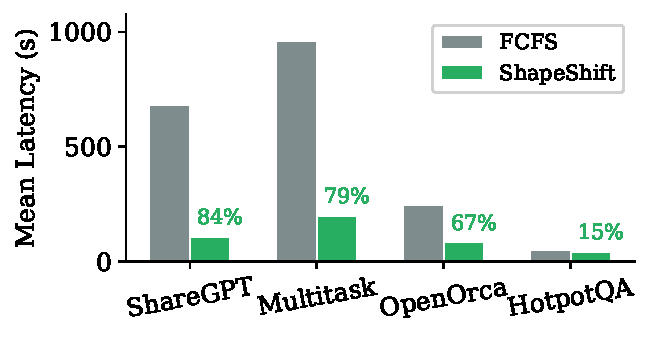
\includegraphics[width=\linewidth]{figures/bar_dinfer_wrapper_mean.pdf}
  \caption{Mean latency}
  \label{fig:dinfer-wrapper-mean}
\end{subfigure}\hfill
\begin{subfigure}[t]{0.3\textwidth}
  \centering
  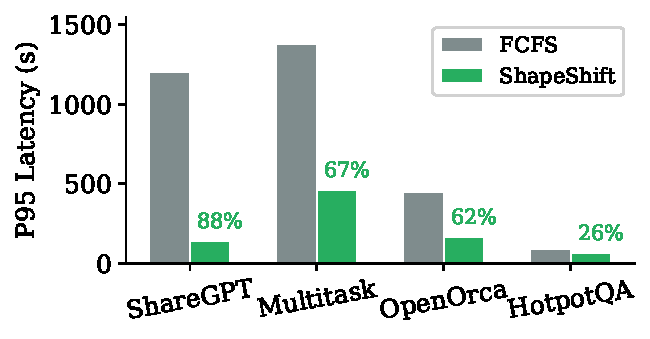
\includegraphics[width=\linewidth]{figures/bar_dinfer_wrapper_p95.pdf}
  \caption{P95 latency}
  \label{fig:dinfer-wrapper-p95}
\end{subfigure}
\caption{dInfer-backed online wrapper results for FCFS and ShapeShift.}
\label{fig:dinfer-wrapper}
\vspace{-0.5em}
\end{figure*}

With the dInfer-backed wrapper, ShapeShift improves online throughput by 1.36--8.41$\times$ across four workloads and reduces p95 latency to 0.12--0.73$\times$ of FCFS. The largest gains appear on long or highly heterogeneous queues, while HotpotQA/Wikipedia shows a smaller gain because the prompt lengths are less fragmented under this trace. These results show that active-shape scheduling can sit above a model-side dLLM acceleration path.

\subsection{Mechanism: Shape Waste Drives the Gain}

The mechanism behind the main result is consistent across workloads: higher FCFS step-level padding ratios expose more scheduling headroom. Table~\ref{tab:stress-tests} makes this relationship explicit with synthetic length traces that keep the serving configuration fixed while widening the prompt-length distribution. ``FCFS pad'' and ``Policy pad'' are mean rectangular padding ratios, and the last two columns normalize throughput and p95 latency to FCFS on the same trace. As length heterogeneity increases, FCFS step padding rises from 1.06$\times$ to 2.09$\times$, and ShapeShift throughput gain rises from 1.08$\times$ to 2.31$\times$.

This trend matches the expected boundary behavior. When lengths are similar, FCFS already forms reasonably compact rectangles and the scheduler has little extra shape structure to exploit. As length spread grows, arrival order becomes a worse proxy for compatible co-residence, and FCFS pays more rectangular padding. ShapeShift reduces this padding by selecting companions around a local length region, so both throughput and tail latency improve in the same regime where the measured shape-padding ratio improves.

\subsection{Ablation: Scheduler Components}

Figure~\ref{fig:ablation} separates the design choices on the main LLaDA-8B online serving matrix. ShapeShift-Shape captures the utilization gain from nearest-length active-shape batching. ShapeShift-Aging adds service-gap control on top of shape batching. Full ShapeShift adds compactness filtering, giving the scheduler explicit runtime controls for both padding and service gaps.

\begin{figure*}[t]
\centering
\begin{subfigure}[t]{0.3\textwidth}
  \centering
  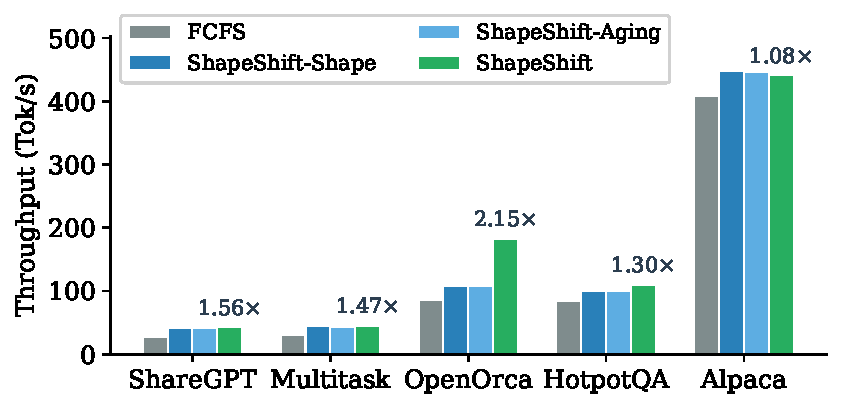
\includegraphics[width=\linewidth]{figures/bar_llada8b_ablation_throughput.pdf}
  \caption{Throughput}
  \label{fig:ablation-throughput}
\end{subfigure}\hfill
\begin{subfigure}[t]{0.3\textwidth}
  \centering
  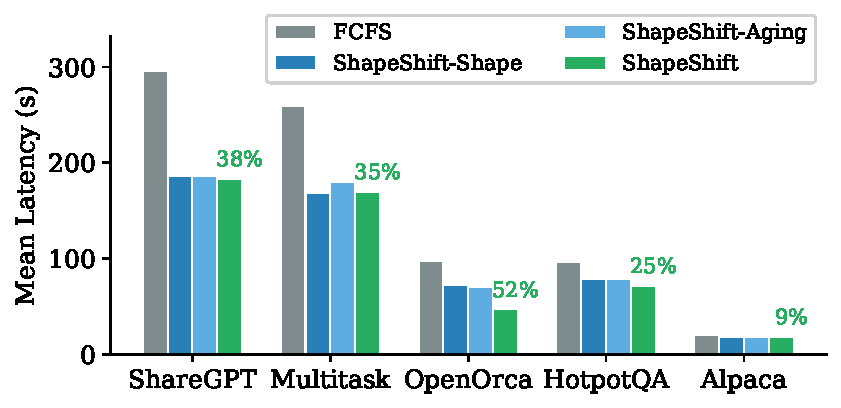
\includegraphics[width=\linewidth]{figures/bar_llada8b_ablation_mean.pdf}
  \caption{Mean latency}
  \label{fig:ablation-mean}
\end{subfigure}\hfill
\begin{subfigure}[t]{0.3\textwidth}
  \centering
  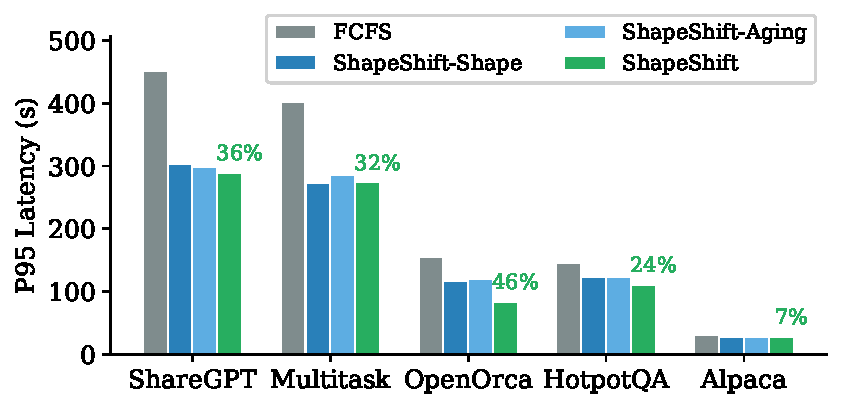
\includegraphics[width=\linewidth]{figures/bar_llada8b_ablation_p95.pdf}
  \caption{P95 latency}
  \label{fig:ablation-p95}
\end{subfigure}
\caption{Scheduler ablation on LLaDA-8B across five mixed-length serving workloads.}
\label{fig:ablation}
\vspace{-0.5em}
\end{figure*}

Table~\ref{tab:stress-tests} also stresses the service-regularity path using a bimodal queue with short, medium, and long outlier requests and a stricter service-gap setting. Shape-only batching reduces padding and improves throughput; aging and the full ShapeShift policy further reduce request latency. In the same service stress, p95 inter-service wait drops from 142.7s under FCFS to 62.3s with ShapeShift-Shape, 67.3s with ShapeShift-Aging, and 57.9s with full ShapeShift.

\begin{table}[t]
\centering
\scriptsize
\setlength{\tabcolsep}{2.5pt}
\resizebox{\columnwidth}{!}{%
\begin{tabular}{llrrrr}
\toprule
Stress & Setting / Policy & FCFS pad & Policy pad & Tput/FCFS & P95/FCFS \\
\midrule
Heterogeneity & Low-CV trace & 1.06 & 1.03 & 1.08$\times$ & 0.93 \\
Heterogeneity & Medium-CV trace & 1.57 & 1.11 & 1.91$\times$ & 0.52 \\
Heterogeneity & High-CV trace & 2.09 & 1.21 & 2.31$\times$ & 0.43 \\
\midrule
Service & ShapeShift-Shape & 2.39 & 1.62 & 1.71$\times$ & 0.58 \\
Service & ShapeShift-Aging & 2.39 & 1.37 & 2.13$\times$ & 0.47 \\
Service & ShapeShift & 2.39 & 1.37 & 2.14$\times$ & 0.47 \\
\bottomrule
\end{tabular}
}
\caption{Shape-heterogeneity and service-regularity stress tests in dlmserve.}
\label{tab:stress-tests}
\end{table}

The effect persists on a longer online serving path. Figure~\ref{fig:fullstep} repeats the validation on five workloads. ShapeShift-Shape improves throughput by 1.14--1.88$\times$ and reduces p95 latency to 0.53--0.88$\times$ of FCFS. ShapeShift-Aging keeps most of the throughput gain while adding an explicit service-gap knob. Offline length-sorted scheduling provides a headroom reference by grouping requests with future length knowledge.

\begin{figure}[t]
\centering
\begin{subfigure}[t]{\linewidth}
  \centering
  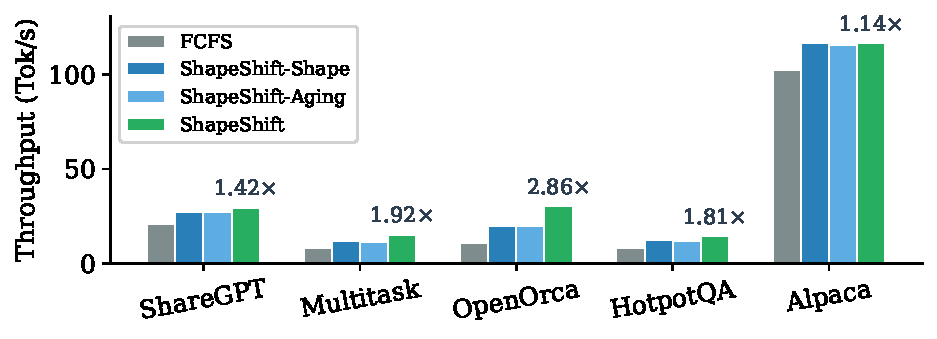
\includegraphics[width=0.9\linewidth]{figures/bar_llada8b_fullstep_throughput.pdf}
  \caption{Throughput}
  \label{fig:fullstep-throughput}
\end{subfigure}
% \vspace{0.6em}
\begin{subfigure}[t]{0.9\linewidth}
  \centering
  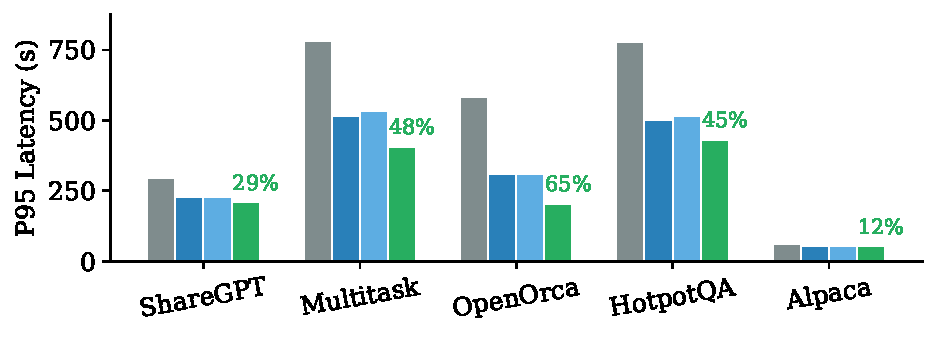
\includegraphics[width=\linewidth]{figures/bar_llada8b_fullstep_p95.pdf}
  \caption{P95 latency}
  \label{fig:fullstep-p95}
\end{subfigure}
\caption{Longer-horizon online validation across five serving workloads.}
\label{fig:fullstep}
\vspace{-0.5em}
\end{figure}

\subsection{Sensitivity and Boundary Cases}

Backlog sensitivity follows the shape-waste mechanism. On the ShareGPT multiturn trace with all requests ready, ShapeShift-Shape and ShapeShift-Aging improve throughput by 1.37$\times$ and 1.30$\times$ while reducing p95 latency to 0.73$\times$ and 0.77$\times$ of FCFS. When arrivals are spread by 100--500ms, the ready pool becomes thin and both policies converge to FCFS, with throughput within 0.99--1.02$\times$ and p95 latency within 0.98--1.04$\times$. This behavior places ShapeShift in the backlogged, shape-diverse long-context regime where active step-batch selection has room to act.

\section{Limitations and Scope}

ShapeShift targets online text dLLM queues where the ready pool is both backlogged and length-heterogeneous. This is the regime in which repeated transformer-shape padding becomes a scheduling resource: many requests are ready at the same time, and FCFS can repeatedly pair short contexts with long ones. Under thin offered load or narrow prompt-length distributions, the ready pool contains fewer shape-compatible companions and the gain naturally approaches FCFS.

This paper isolates the single-GPU step-batch decision. A deployment-grade serving system can combine active-shape scheduling with admission control, cluster-level routing, memory placement, and workload-aware autoscaling. Those layers decide when and where requests enter service; ShapeShift decides which active requests share the next dLLM update.

\section{Related Work}

\textbf{LLM serving systems.} Orca~\cite{orca2022}, vLLM~\cite{vllm2023}, DistServe~\cite{distserve2024}, and Sarathi-Serve~\cite{sarathi2024} shape modern LLM-serving evaluation through matched baselines, load sweeps, and throughput under latency constraints. Their scheduling problem is organized around AR prefill/decode, KV-cache residency, and incremental token generation. Length-aware admission and chunked prefill reduce one-time prompt work or decode interference. ShapeShift adopts this methodology, but targets a dLLM cost where length becomes a recurring step-batch resource rather than a prefill attribute.

\textbf{dLLM inference and serving.} Fast-dLLM~\cite{zhao2025fastdllm}, dLLM-Cache~\cite{dllmcache2025}, d$^2$Cache~\cite{d2cache2025}, dKV-Cache~\cite{dkvcache2025}, Sparse-dLLM~\cite{sparsedllm2025}, FOCUS~\cite{focuscompute2026}, and Focus-dLLM~\cite{focusdllm2026} accelerate dLLM inference through cache reuse, sparse attention, or focused computation. dInfer~\cite{dInfer2025}, dLLM-Serve~\cite{dllmserve2025}, vLLM-Omni~\cite{vllmomni2026}, and dlmserve~\cite{dlmserve2026} address dLLM serving and iteration management. These systems reduce the cost of executing a chosen update or managing the update loop; ShapeShift changes the active-set decision that creates the update shape.

\textbf{Diffusion and long-context serving.} DiT-Serve~\cite{ditserve2025}, GenServe~\cite{genserve2026}, and DisagFusion~\cite{disagfusion2026} treat diffusion updates as a serving schedule for image/video workloads. ShapeShift applies this perspective to text dLLMs, where the repeated shape resource is variable sequence-length padding in a bidirectional token transformer. AR long-context systems such as LoongServe~\cite{loongserve2024}, AlignedServe~\cite{alignedserve2026}, and LAPS~\cite{laps2026} also motivate length-aware scheduling, but AR decoding amortizes the prompt through KV-cache reuse and then advances one token at a time.

\textbf{Variable-length dLLM generation.} Length-aware dLLM methods~\cite{nativelength2026} reduce wasted output canvas or improve variable-length generation. Cropping or predicting each request's canvas reduces the per-request length $L_r$; active-shape scheduling reduces padding between heterogeneous requests in the same online batch.

\section{Conclusion}

Long-context dLLM serving introduces a repeated shape-padding problem: short requests batched with long requests pay the long request's transformer shape across repeated denoising updates. ShapeShift treats sequence shape as a step-level scheduling resource, using active-shape batching, compactness filtering, and service-gap aging to recover utilization while preserving service regularity. Direct online dlmserve experiments show 1.19--1.49$\times$ throughput improvement across mixed-length serving workloads, and longer-horizon validation shows 1.14--1.88$\times$ gains. The results point to a simple principle for dLLM serving systems: schedule not only when requests run, but also which sequence shapes run together. As dLLMs move toward longer contexts and shared online service, this active-set decision becomes a first-class part of the serving stack rather than a side effect of arrival order.

\bibliography{references}

\end{document}
